\chapter{Proposed Method}
\label{chap:algorithm}
In this thesis we have implemented a well define digital process to recognize hand writings from a registration form or any kind of forms which are mostly documentation of government or private institutions. Image recognition is a process, which usually consist of taking a picture, process the image then present the results.The whole work can be divided into two parts:
\section{Data Extraction}
We work on a defined format of from. In this process the from every field should be separate by box region.
\begin{figure}[h!]
\centering
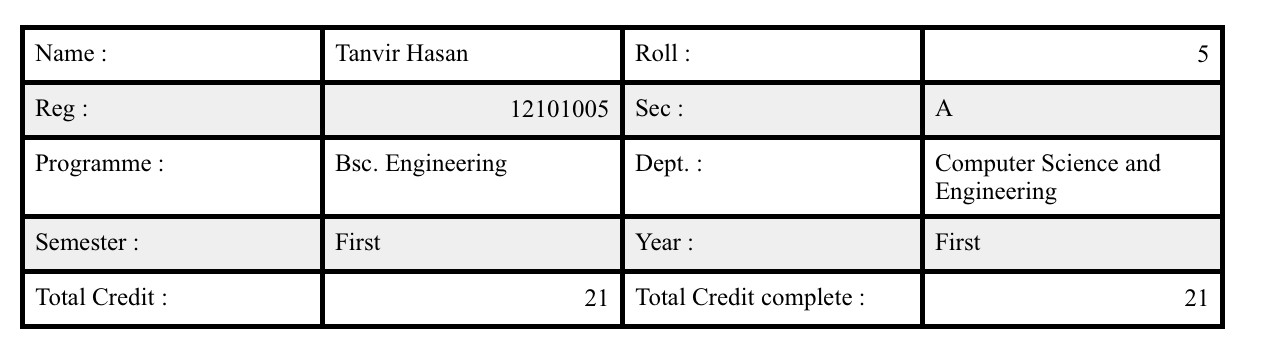
\includegraphics[width=1\textwidth]{from}
\caption {Form template}
\label {fig:FormTemplate}
\end{figure}
\subsection{Convert RGB to Gray Image}
First we have to take input form as picture.Then convert RGB image to gray image.
\begin{figure}[h!]
\centering
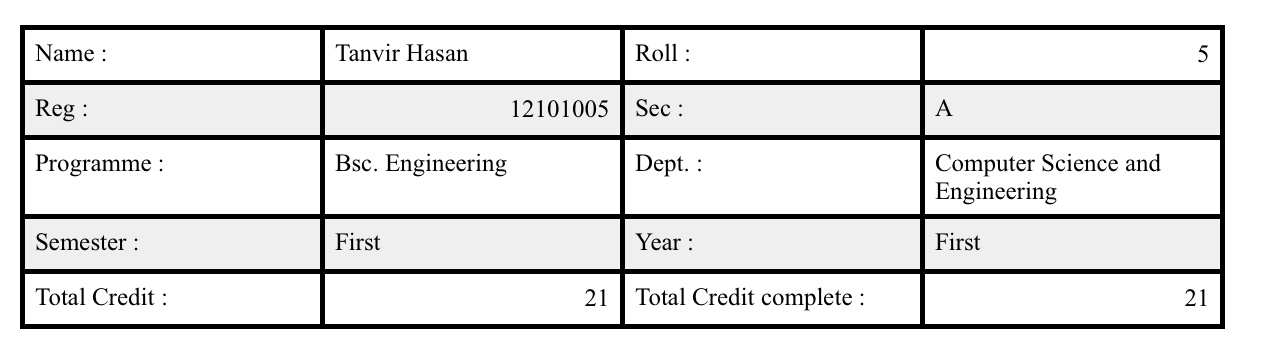
\includegraphics[width=1\textwidth]{GrayImage}
\caption {RGB to Gray}
\label {fig:GRAY}
\end{figure}
\subsection{Image Smoothing}
Smoothing, also called blurring, is a simple and frequently used image processing operation.  There  are  many  reasons  for  smoothing,  but  it  is  usually  done  to  reduce  noise  or  camera artefacts. Smoothing is also important when we wish to reduce the resolution of an image in a principled way\cite{OpenCVBook}.
For our thesis work we used Gaussian blur and this is probably the most useful though not the fastest.
\begin{figure}[h!]
\centering
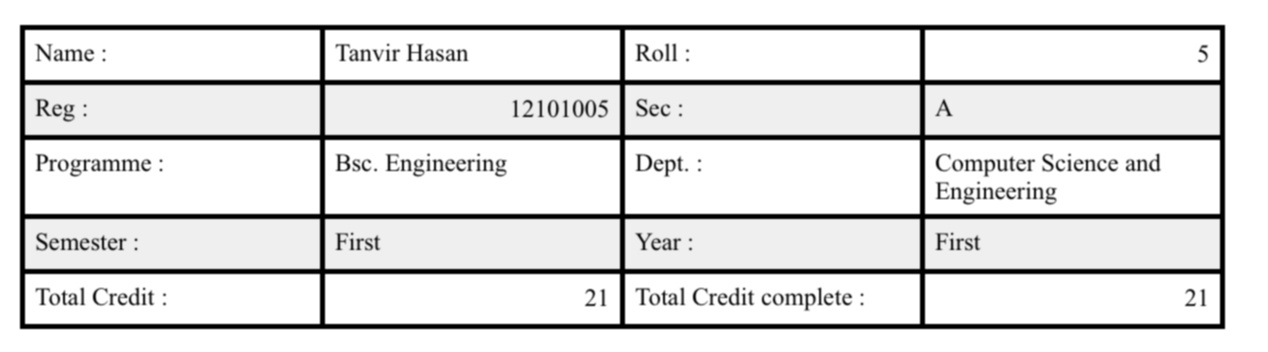
\includegraphics[width=1\textwidth]{GaussianBlur}
\caption {Image after applying gaussian blur in sample form}
\label {fig:GaussianBlur}
\end{figure}
\subsection{Thresholding}
Next we work on image thresholds. Frequently we have done many layers of processing steps and want either to make a final decision about the pixels in an image or to categorically reject those pixels below or above some value while keeping the others. The OpenCV function Threshold() accomplishes these tasks. The basic idea is that an array is given, along with a threshold, and then set a value for every element of the array depending on whether it is below or above the threshold\cite{OpenCVBook}.
\begin{figure}[h!]
\centering
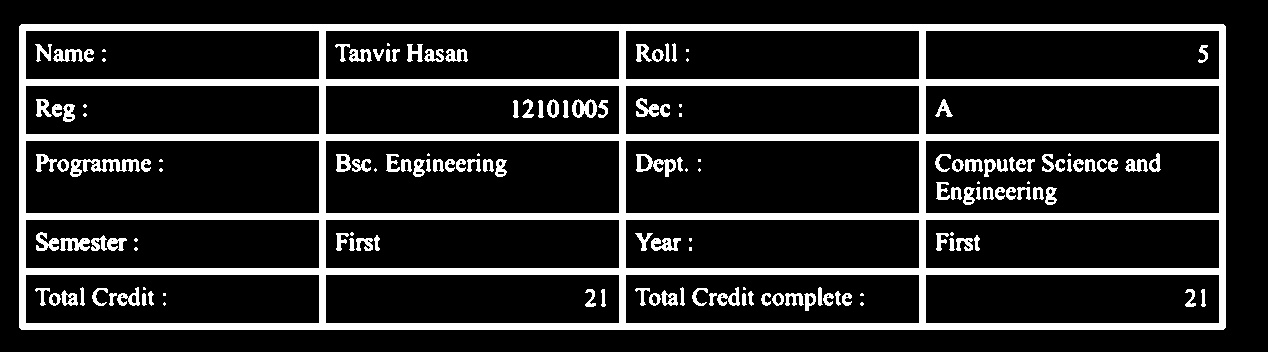
\includegraphics[width=1\textwidth]{Threshold}
\caption {Thresholded image after appling thresholding in sample form}
\label {fig:threshold}
\end{figure}
\subsection{Edge Detection}
We work on the process of edge recognition of an image. For this we used canny edge detector. The method just described in chapter \ref{EdgeDitectionR} for finding edges. The Canny()  function expects an input image, which must be gray scale, and an output image, which must also be gray scale (but which will actually be a Boolean image).\cite{OpenCVBook}
\begin{figure}[h!]
\centering
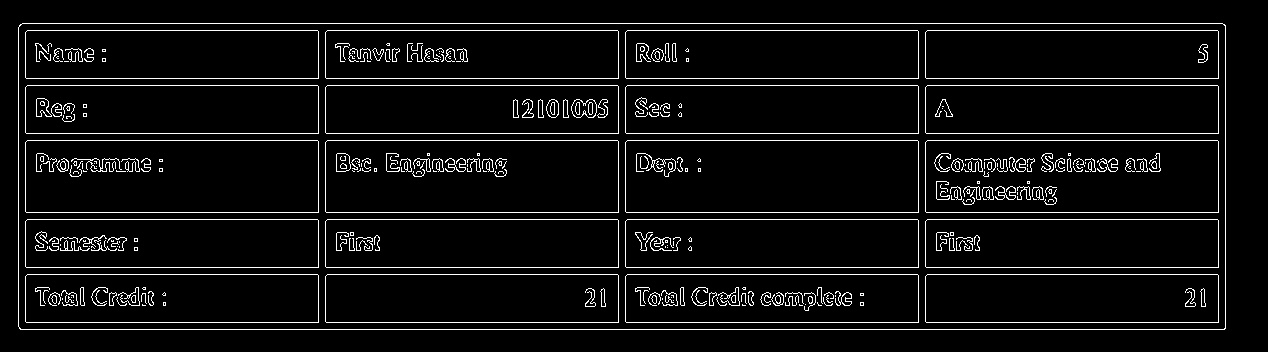
\includegraphics[width=1\textwidth]{Canny2}
\caption {Canny Edge detected image after applying canny edge detection in sample form}
\label {fig:Canny}
\end{figure}
\subsection{Finding Contour}
After edge detection we find out the contours on these defined edges. For this we using opencv function findContours().
\subsection{Select only rectangle shape region}
There can be many regular and irregular shape of contours. But we need only rectangular shape contour. After find contours we filter out irregular shape and keep only the rectangular shape contours. In the \ref{Shape} section we describe how to find rectangle shape.
\subsection{Store only unique region}
For thicker edge one region can be occur multiple time. For this reason we need to filter out only unique region. To doing this we map these region with their left most point coordinate x,y. In every selected left most x,y coordinate we must find unique rectangle region. This is the most efficient way. Otherwise mapping whole region point will be costly.
\subsection{Mapping From Field and Value}
For mapping from different type of field with value, we first store every unique region left-upper most x,y 2D point. Then we sort these 2D point respectively y coordinate then x coordinate. Then we take pair of region form sorted region. The first element of pair will be from filed and second field will be value.
\section{Data Reorganization}
After extracting data from an analogue image, we work on recognize our extracted data by using Tesseract open source engine.  Tesseract converts  the  input  image  into  binary  format  using thresholding. Outlines of  components are  stored  on  connected component   analysis.   Nesting   of   outlines   is   done   which gathers  the  outlines  together  to  form  a  Blob. Text  lines  are analyzed  for  fixed  pitch  and  proportional  text.  Then  the  lines are  broken  into  words  by  analysis  according  to  the  character spacing.   Fixed pitch   is chopped   in   character   cells   and proportional  text  is  broken  into  words  by  definite  spaces  and fuzzy spaces\cite{OCR}.

Tesseract recognises a word in two passes, one is tries  to recognize  the  words in  the  first  pass. If  the  match  is found, then  the  found word  is  passed on to the qdaptive  classifier, which recognizes the text more accurately. During the second pass, the  words  which  were  not at  all recognized or  were  not well recognized in the first pass are recognized again through a run  over through the  page.  Finally  Tesseract  resolves  fuzzy spaces.  To locate  small  and  capital  text, Tesseract  checks alternative hypothesis for x-height OCR engine\cite{OCR} \cite{TesseractORCEngineOfficialWeb}.
\section{Tesseract Training}
For better accuracy we need to train tesseract OCR engine with different type of data.\\
The training procedure of tesseract is well describe in official website of tesseract\cite{TrainingTesseract}\cite{OCR}. 
In short, the training step go through these following steps:
\begin{enumerate}
\item Generate Training Images
\item Make Box Files
\item Edit Box Files
\item Run Tesseract for Training
\item Compute the Character Set
\item set unicharset properties
\item font properties
\item Clustering
\item Putting it all together and make tessdata file.
\end{enumerate}